\chapter{Especificação de requisitos do trabalho}

\label{CAP4}


% definir técnicas, processos e sistemas, procedimentos que vão compor o sistema

Neste capítulo serão descritas as necessidades básicas levantadas para que o projeto funcione como esperado.

Na figura \ref{fig:class_diagram} pode ser visto o diagrama de classes que define o sistema como um todo.

\begin{figure}[hp]
    \centering
    
    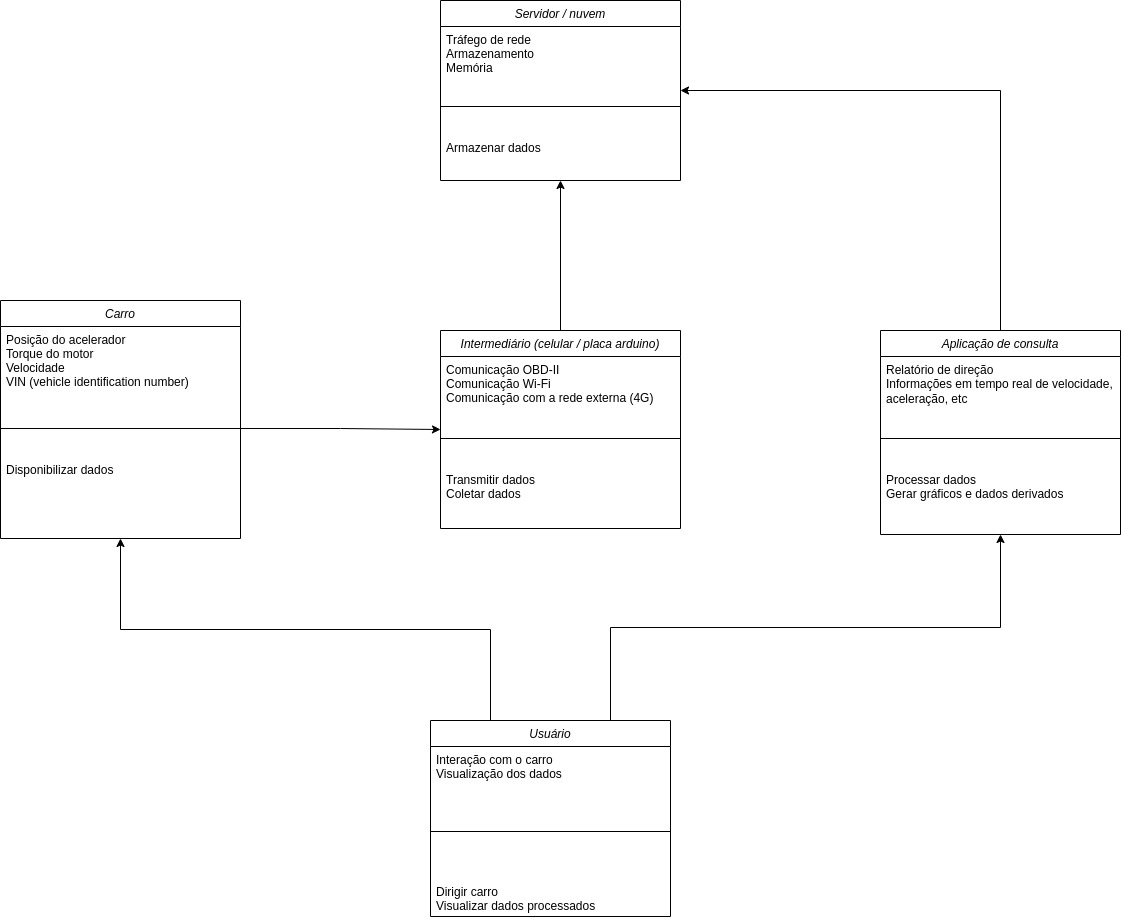
\includegraphics[scale=0.4]{figures/coleta_dados_carro}
    
    \caption{Diagrama de classes com visão mais abstrata do sistema}
    
    \label{fig:class_diagram}
\end{figure}

\section{Requisitos funcionais}
\begin{itemize}
    \item \textbf{Comunicação OBD-II:} o aplicativo faz comunicação com a interface do carro, requisitando apenas as informações definidas, durante o projeto, como relevantes.
    
    \item \textbf{Conexão do celular à \textit{internet}:} usando-se a tecnologia 4G, deve ser responsável por mandar os dados coletados para a nuvem.
    
    \item \textbf{Plataforma de recepção na nuvem:} os dados brutos coletados do carro e do celular (GPS e acelerômetro), assim como as informações depois já processadas, serão todos armazenados na plataforma de \textit{cloud} definida.
    
    \item \textbf{Histórico de Rotas:} o sistema deve ter a capacidade de armazenar e acessar informações detalhadas sobre os trajetos percorridos por um veículo ao longo do tempo. Este recurso é crucial para oferecer aos usuários e administradores uma visão retrospectiva das atividades de um veículo, permitindo uma compreensão abrangente dos padrões de movimentação e comportamento de condução.
\end{itemize}

\section{Requisitos não-funcionais}

\begin{itemize}
    \item \textbf{Conexão contínua com a \textit{internet}:} caso a conexão pare por muito tempo, a análise dos dados coletados pode ser prejudicada, além de gerar desconfiança por parte do usuário, ao perceber que não há consistência no sistema.
    
    \item \textbf{Interface sem reconexão manual com a \textit{internet} e \textit{bluetooth}:} se o sistema desligar, a conexão com o OBD e com a \textit{internet} deve ser re-estabelecida sem interferência do usuário assim que for ligada novamente; em outras palavras, o sistema deve ser o mais \textit{plug and play} possível.
    
    \item \textbf{Informações relevantes e corretas:} os dados apresentados no relatório de direção precisam ter sentido para o usuário; meta-informações são as únicas que devem chegar até o usuário final, e também precisam passar por algum tipo de "filtro de plausibilidade", para que, mais uma vez, a confiança de quem usará o sistema não seja perdida ao deparar-se com valores \textit{outliers} nas análises geradas.
    
    \item \textbf{Memória e armazenamento em nuvem suficientes:} o espaço máximo em nuvem que pode ser usado deve ficar claro para o usuário quando ele usar o sistema; o motorista precisa ficar ciente de que suas informações não serão mais coletadas assim que o armazenamento seja ocupado por completo.
    
    \item \textbf{Segurança de dados:} pessoas não-autorizadas não pode ter acesso aos dados coletados no veículo de cada usuário.
\end{itemize}

% \subsection{}
% \subsection{}
% \subsection{}


